% !TEX root = ../Seminararbeit-Data_Mining_Frameworks.tex
%


% =============================================================================
%
% Datensatz und Beispiel-Modell
%
% =============================================================================
\chapter{Datensatz und Beispiel-Modell}
\label{sec:example}

\section{Datensatz}
\label{sec:example:data}

\begin{figure}[htb]
	
\includegraphics[width=\textwidth]{gfx/crisplinear.png}
	\caption{Der CRISP-DM Prozess als Kette der einzelnen Schritte}
	\label{fig:example:data:crisp}
\end{figure}

Für die Umsetzung des Beispiels wurde der Eingangs bereits beschriebene CRISP-DM
Data Mining Prozess verwendet. Die Daten wurden gemäß den 6 Schritten „Business
Understanding“, „Data Understanding“, „Data Preparation“, „Modeling“,
„Evaluation“ und „Deployment“ verarbeitet.

\subsection{Business Understanding}
\label{sec:example:data:bu}

Als Datengrundlage für das Beispiel dienen die Daten der
Veranstaltungsevaluationen der Vergangenen Semester, durchgeführt von der
Fachschaft Mathematik, Physik und Informatik der Universität Bayreuth. Mithilfe
der vorliegenden Datengrundlage sollen nun folgende Fragen beantwortet werden:

\begin{itemize}
  \item „Warum beschweren sich einige Studenten, während andere die Veranstaltung
  super finden? Bzw. welche Ursachen gibt es für eine Beschwerde?“
  \item „Wie sind die Prognosen für die bevorstehenden Evaluationen?“
\end{itemize}

\subsection{Data Understanding}
\label{sec:example:data:du}

Im nächsten Schritt ist es wichtig herauszufinden, wie die Daten erhoben wurden.
Im Beispiel der Veranstaltungsevaluationen ist dies durch Austeilen eines
Fragebogens erfolgt.

\begin{figure}[htb]
	
\includegraphics[width=\textwidth]{gfx/questionnaire.png}
	\caption{Fragebogen, zur Erhebung der Evaluationsdaten}
	\label{fig:example:data:du:qu}
\end{figure}

Anhand des Fragebogens erkennt man, dass die Antwortmöglichkeiten in Form von
anzukreuzenden Kästchen gegeben waren. Jedes Kreuz repräsentiert dabei einen
Wert im Bereich von 0 bis max. 4. \\
Außerdem muss festgestellt werden, wie die Daten in der Datenbank abgelegt
werden. Hierfür kann man bspw. ein ER-Diagramm erzeugen oder sich eine Vorschau
der Daten in Form einer Tabelle generieren lassen.

\begin{figure}[htb]
  \center
	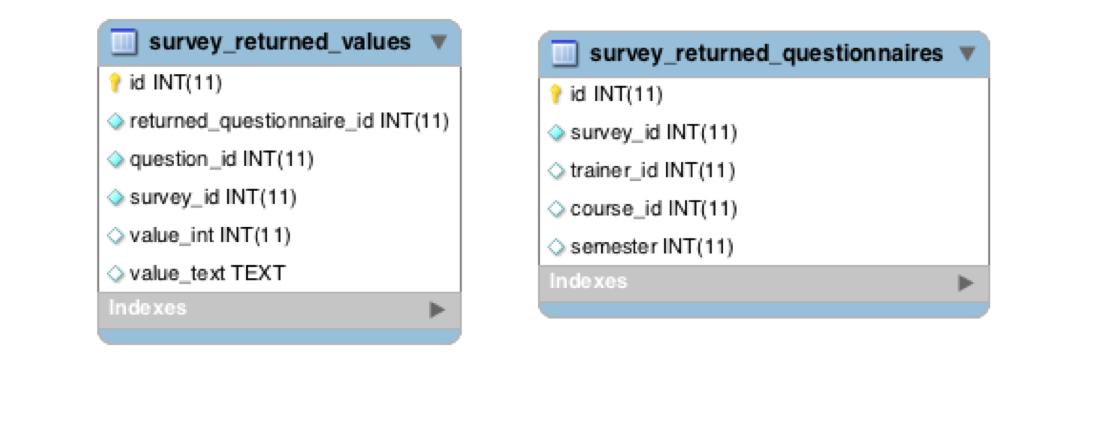
\includegraphics[width=0.7\textwidth]{gfx/db1.png}
  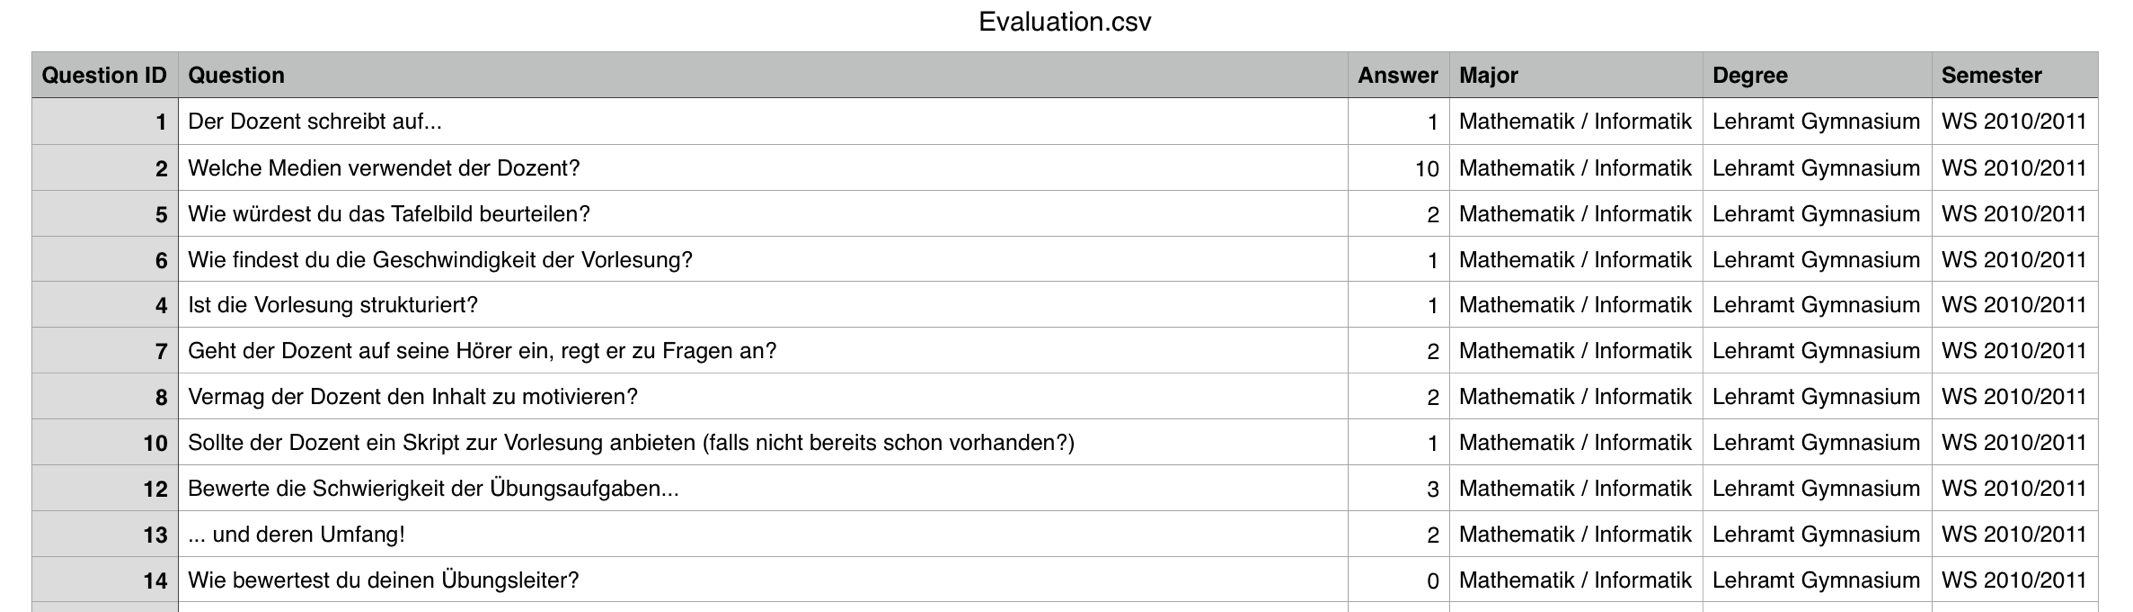
\includegraphics[width=\textwidth]{gfx/db2.png}
	\caption{Repräsentation der Daten in der Datenbank}
	\label{fig:example:data:du:db}
\end{figure}

Mithilfe dieser Informationen erkennt man, dass sich die gesuchten Daten in den
beiden Tabellen „survey\_returned\_values“ und „survey\_returned\_questionnaires“
befinden und wie diese strukturiert sind.

\subsection{Data Preparation}
\label{sec:example:data:dp}

Wurden nun die entsprechenden Tabellen bzw. deren Attribute festgelegt, müssen
diese nun im nächsten Schritt aus der Datenbank extrahiert werden, um separat
Analysiert werden zu können. Dies geschieht mit der folgenden SQL-Abfrage.

\begin{figure}[htb]
	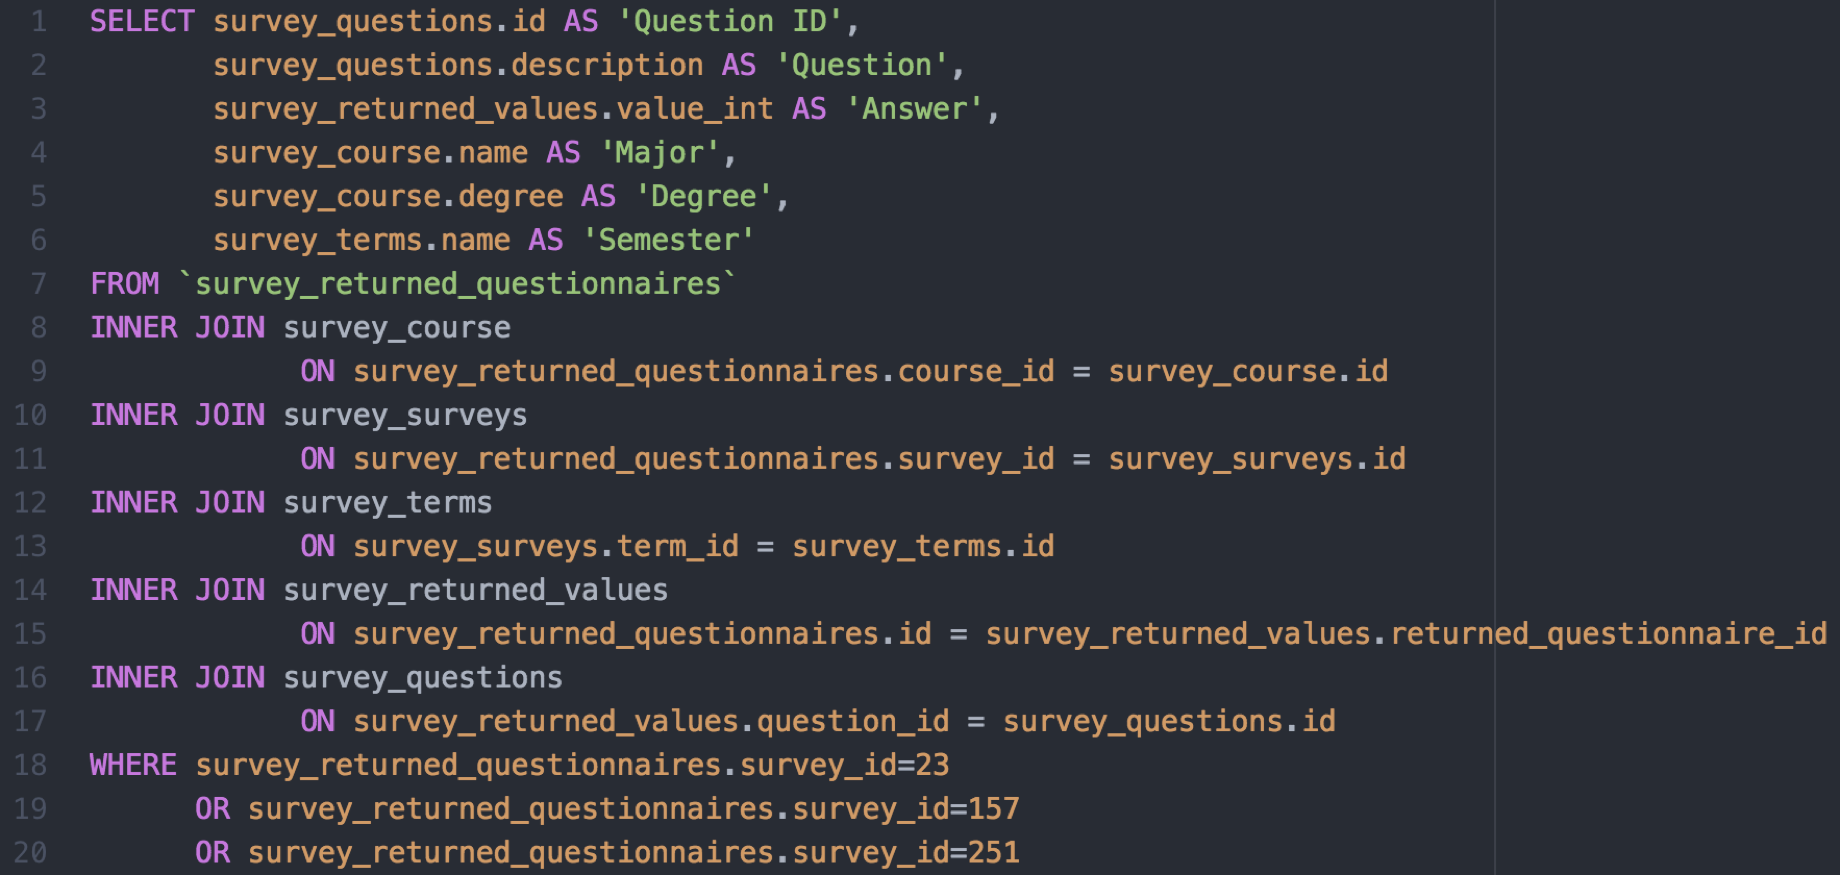
\includegraphics[width=\textwidth]{gfx/sql.png}
	\caption{SQL Anfrage für den Export der Daten}
	\label{fig:example:data:dp:sql}
\end{figure}

Die Ergebnisdatensätze der SQL-Abfrage können nun als .csv Datei exportiert
werden, um danach in der jeweiligen Data Mining Software verarbeitet werden zu
können.

\subsection{Modeling}
\label{sec:example:data:mod}

In der Modellierungsphase muss nun ein Algorithmus gewählt werden, welcher die
vorbereiteten Daten so verarbeiten kann, dass die definierten
Fragestellungen beantwortet werden können. In unserem Beispiel eignet sich die
Frage nach der Gesamtnote, da dieses Attribut eine gute Repräsentation der
Gesamtbewertung für eine Veranstaltung darstellt. \\
Es muss also ein Algorithmus gewählt werden, welcher nach einem einzelnen
Attribut, dem sog. Label, Daten Mined. Ein einfach auszuwertender Algorithmus,
der genau diese Voraussetzungen erfüllt ist der sog. „Entscheidungsbaum“
(engl.: „Decision Tree“).

\begin{figure}[htb]
  \center
	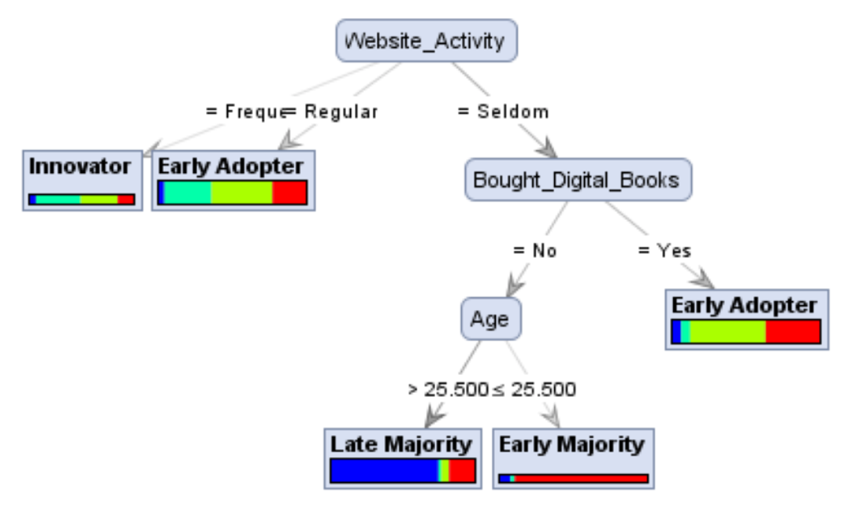
\includegraphics[width=0.5\textwidth]{gfx/dt.png}
	\caption{Beispiel für einen Entscheidungsbaum \cite{North:2012}}
	\label{fig:example:data:mod:dt}
\end{figure}

Die Knoten des Baumes stellen klassifizierende Attribute des Ausgangs-Datensatzes
dar, während die Blätter die möglichen Werte des Labels anzeigen. Außerdem
zeigen die Blätter noch an, auf wieviel Datensätzen die jeweilige Klasse beruht.

\subsection{Evaluation + Deployment}
\label{sec:example:data:eval}

Schließlich kann mithilfe des „Decision Trees“ ermittelt werden, dass
beispielsweise das Studienfach oder ein bestimmtes Semester die Ursache für
vermehrte Beschwerden (respektive mehrere schlechte Bewertungen) waren.
Gleichzeitig kann man mit den entsprechenden Informationen über Studienfach,
Abschluss etc. der aktuellen Kursteilnehmer eine Prognose für die bevorstehende
Lehrveranstaltungsevaluation abgeben.

\section{Umsetzung}
\label{sec:example:impl}

\subsection{Rapidminer Studio}
\label{sec:example:impl:rm}

Um das Beispielszenario in RapidMiner Studio umzusetzen wurde der folgende
Prozess modelliert:

\begin{figure}[htb]
  \center
	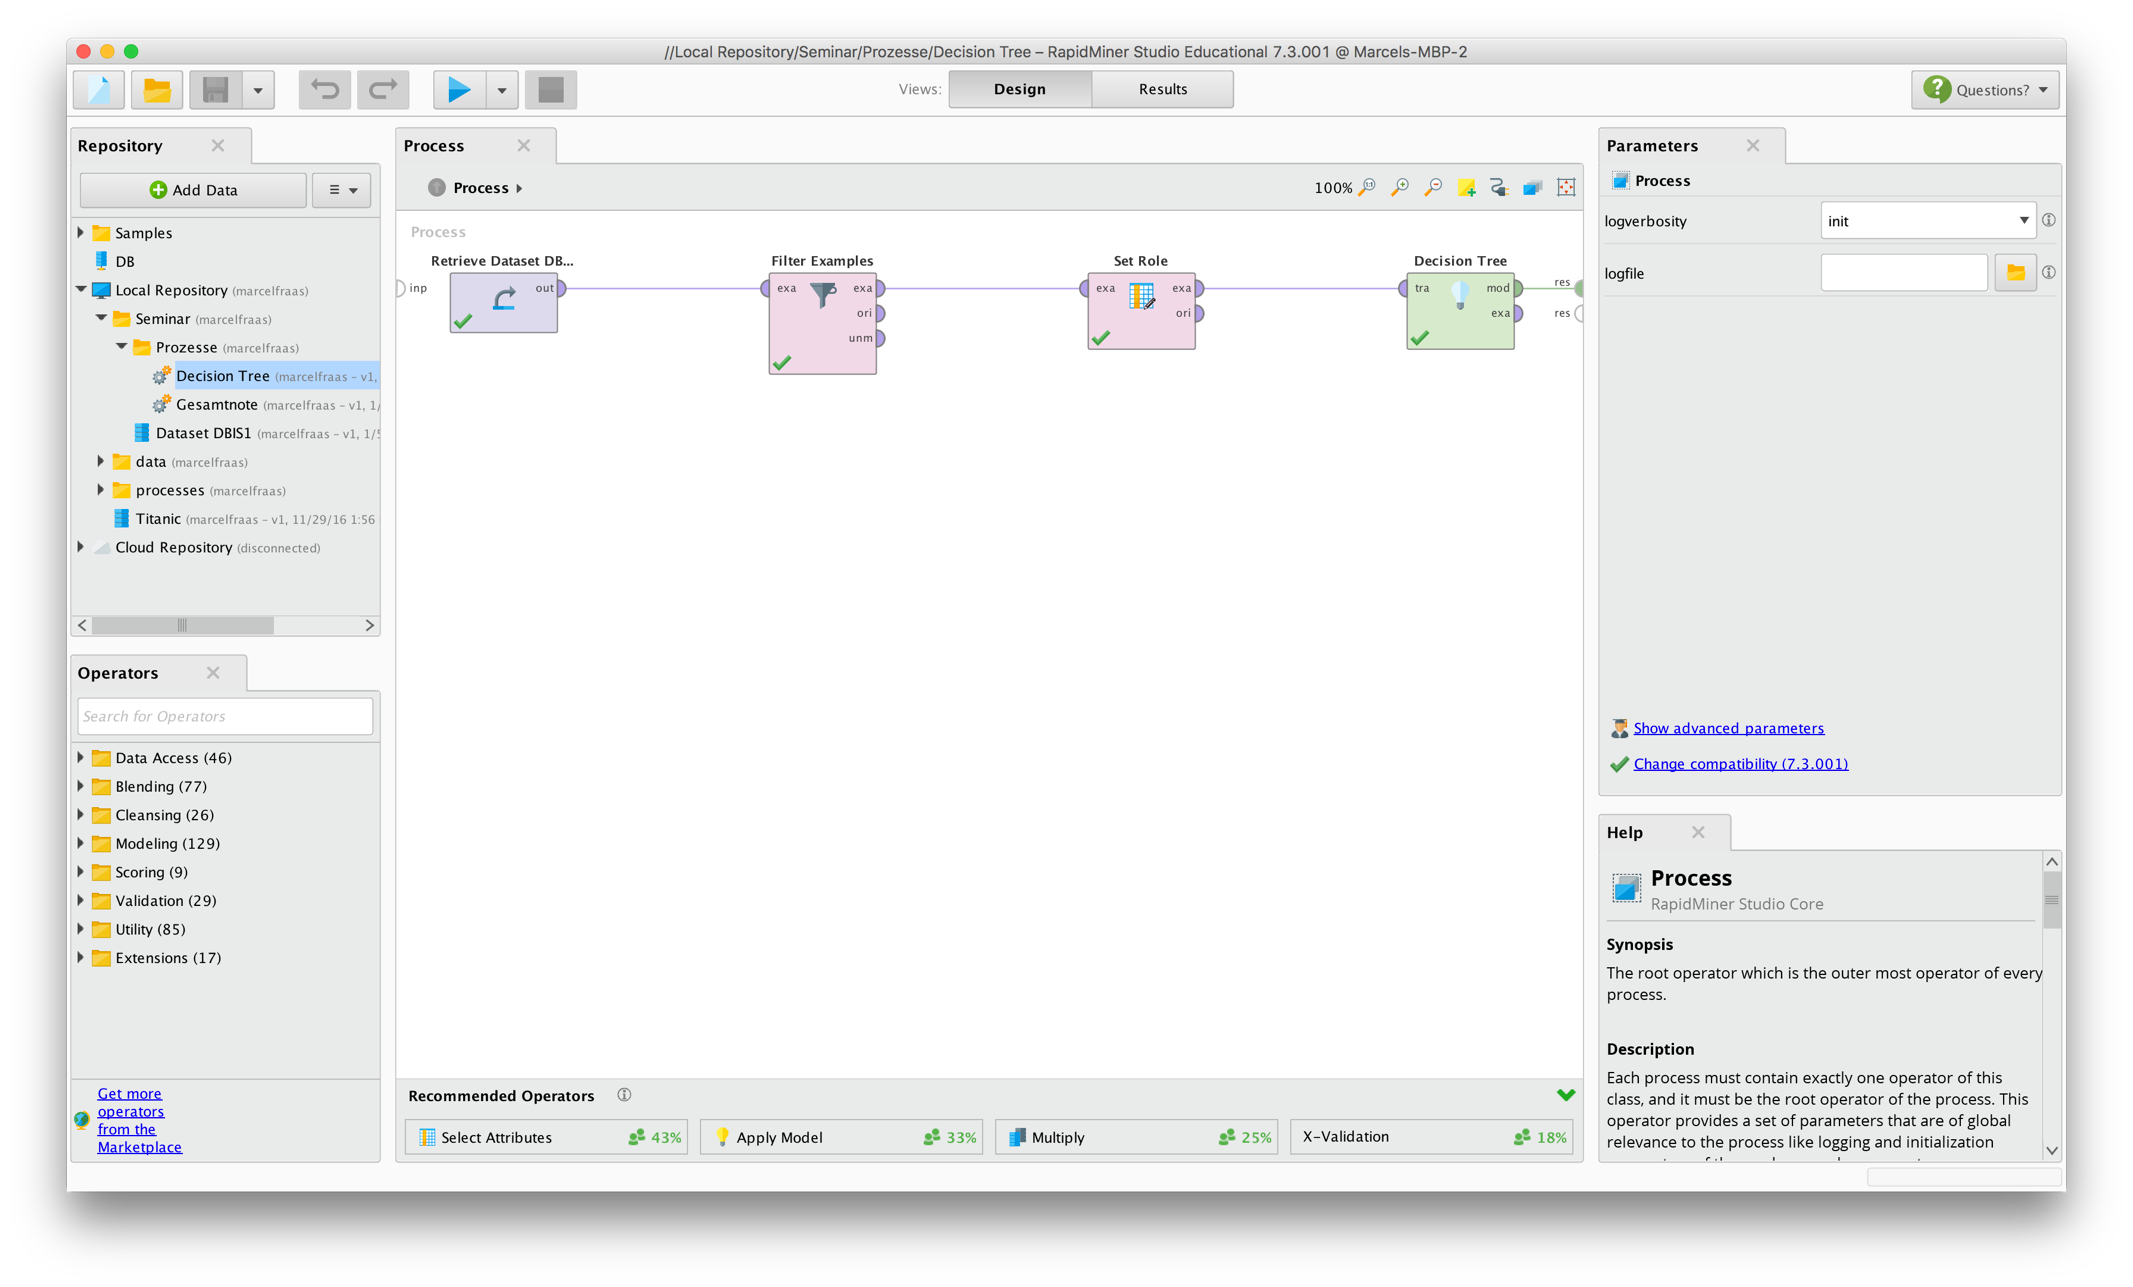
\includegraphics[width=0.9\textwidth]{gfx/rmproc.png}
	\caption{Der Beispielprozess im RapidMiner Studio}
	\label{fig:example:impl:rm:proc}
\end{figure}

Zunächst wurde die .csv Datei mit dem „Retrieve Dataset“ Operator in den Prozess
geladen. Anschließend wurden per „Filter Example“ sowohl alle Datensätze mit
NULL Einträgen entfernt, als auch die Einträge, welche die Frage nach der
Gesamtnote beinhalten, extrahiert. Danach wurde die Spalte „Answer“, welche den
Wert der Note beinhaltet als „Label“ definiert. Zuletzt wurden die Daten dann
dem „Decision Tree“ Algorithmus übergeben und das Ergebnis zurück in die Anzeige
geladen.

\begin{figure}[htb]
	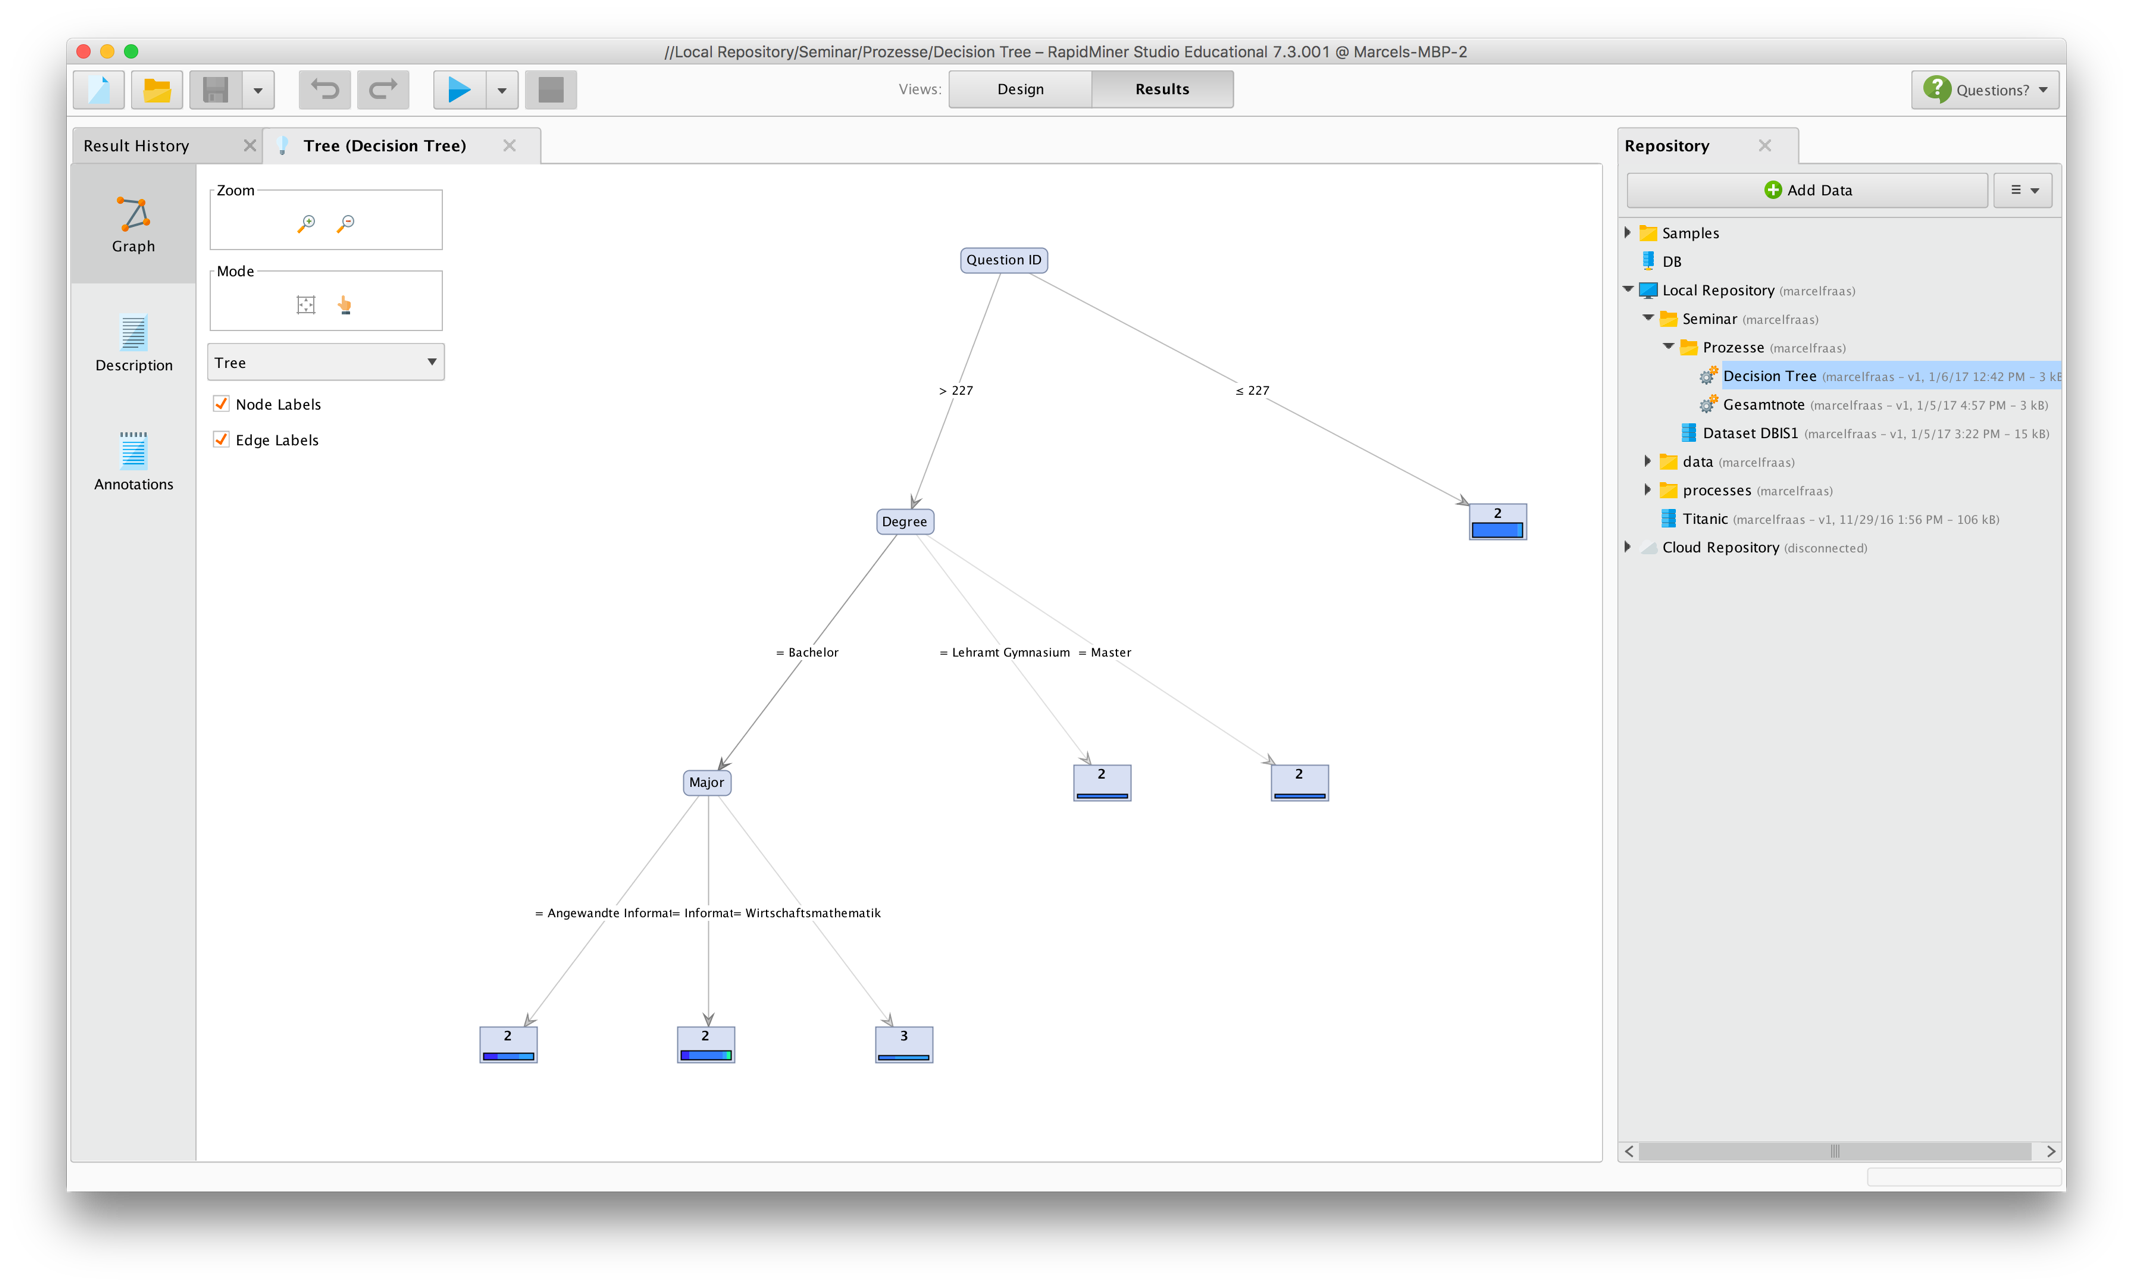
\includegraphics[width=\textwidth]{gfx/rmres.png}
	\caption{Das Ergebnis im RapidMiner Studio}
	\label{fig:example:impl:rm:res}
\end{figure}

Das Ergebnis ist ein Baum, an welchem erkennbar ist, dass in den meisten Fällen
die Note „2“ für die Lehrveranstaltung vergeben wurde. Einzig bei der
Betrachtung des Studienfaches fällt auf, dass Studierende, welche dem „Major“
Wirtschaftsmathematik angehören, eine 3 vergeben haben. An den Blättern lässt
sich außerdem ablesen, wie groß die sog. „Confidence“ ist, also auf wie vielen
Daten, die jeweilige Entscheidung basiert. Kenntlich gemacht wird dies durch
die jeweiligen farblichen Balken. Diese sind wie folgt zu interpretieren: Je
dicker (höher) der Balken, desto mehr Datensätze liegen der Entscheidung
zugrunde. Anhand (der Anzahl) der Farben erkennt man wieviel unterschiedliche
Werte für die jeweilige Klasse gefunden wurden, und entsprechend an der „breite“
der Farbe kann man ablesen, wie oft der jeweilige Wert in Relation aufgetaucht
ist.

\subsection{Microsoft Azure Machine Learning Studio}
\label{sec:example:impl:msa}

Das korrespondierende Experiment im Microsoft Azure Machine Learning Studio
sieht folgendermaßen aus:

\begin{figure}[htb]
  \center
	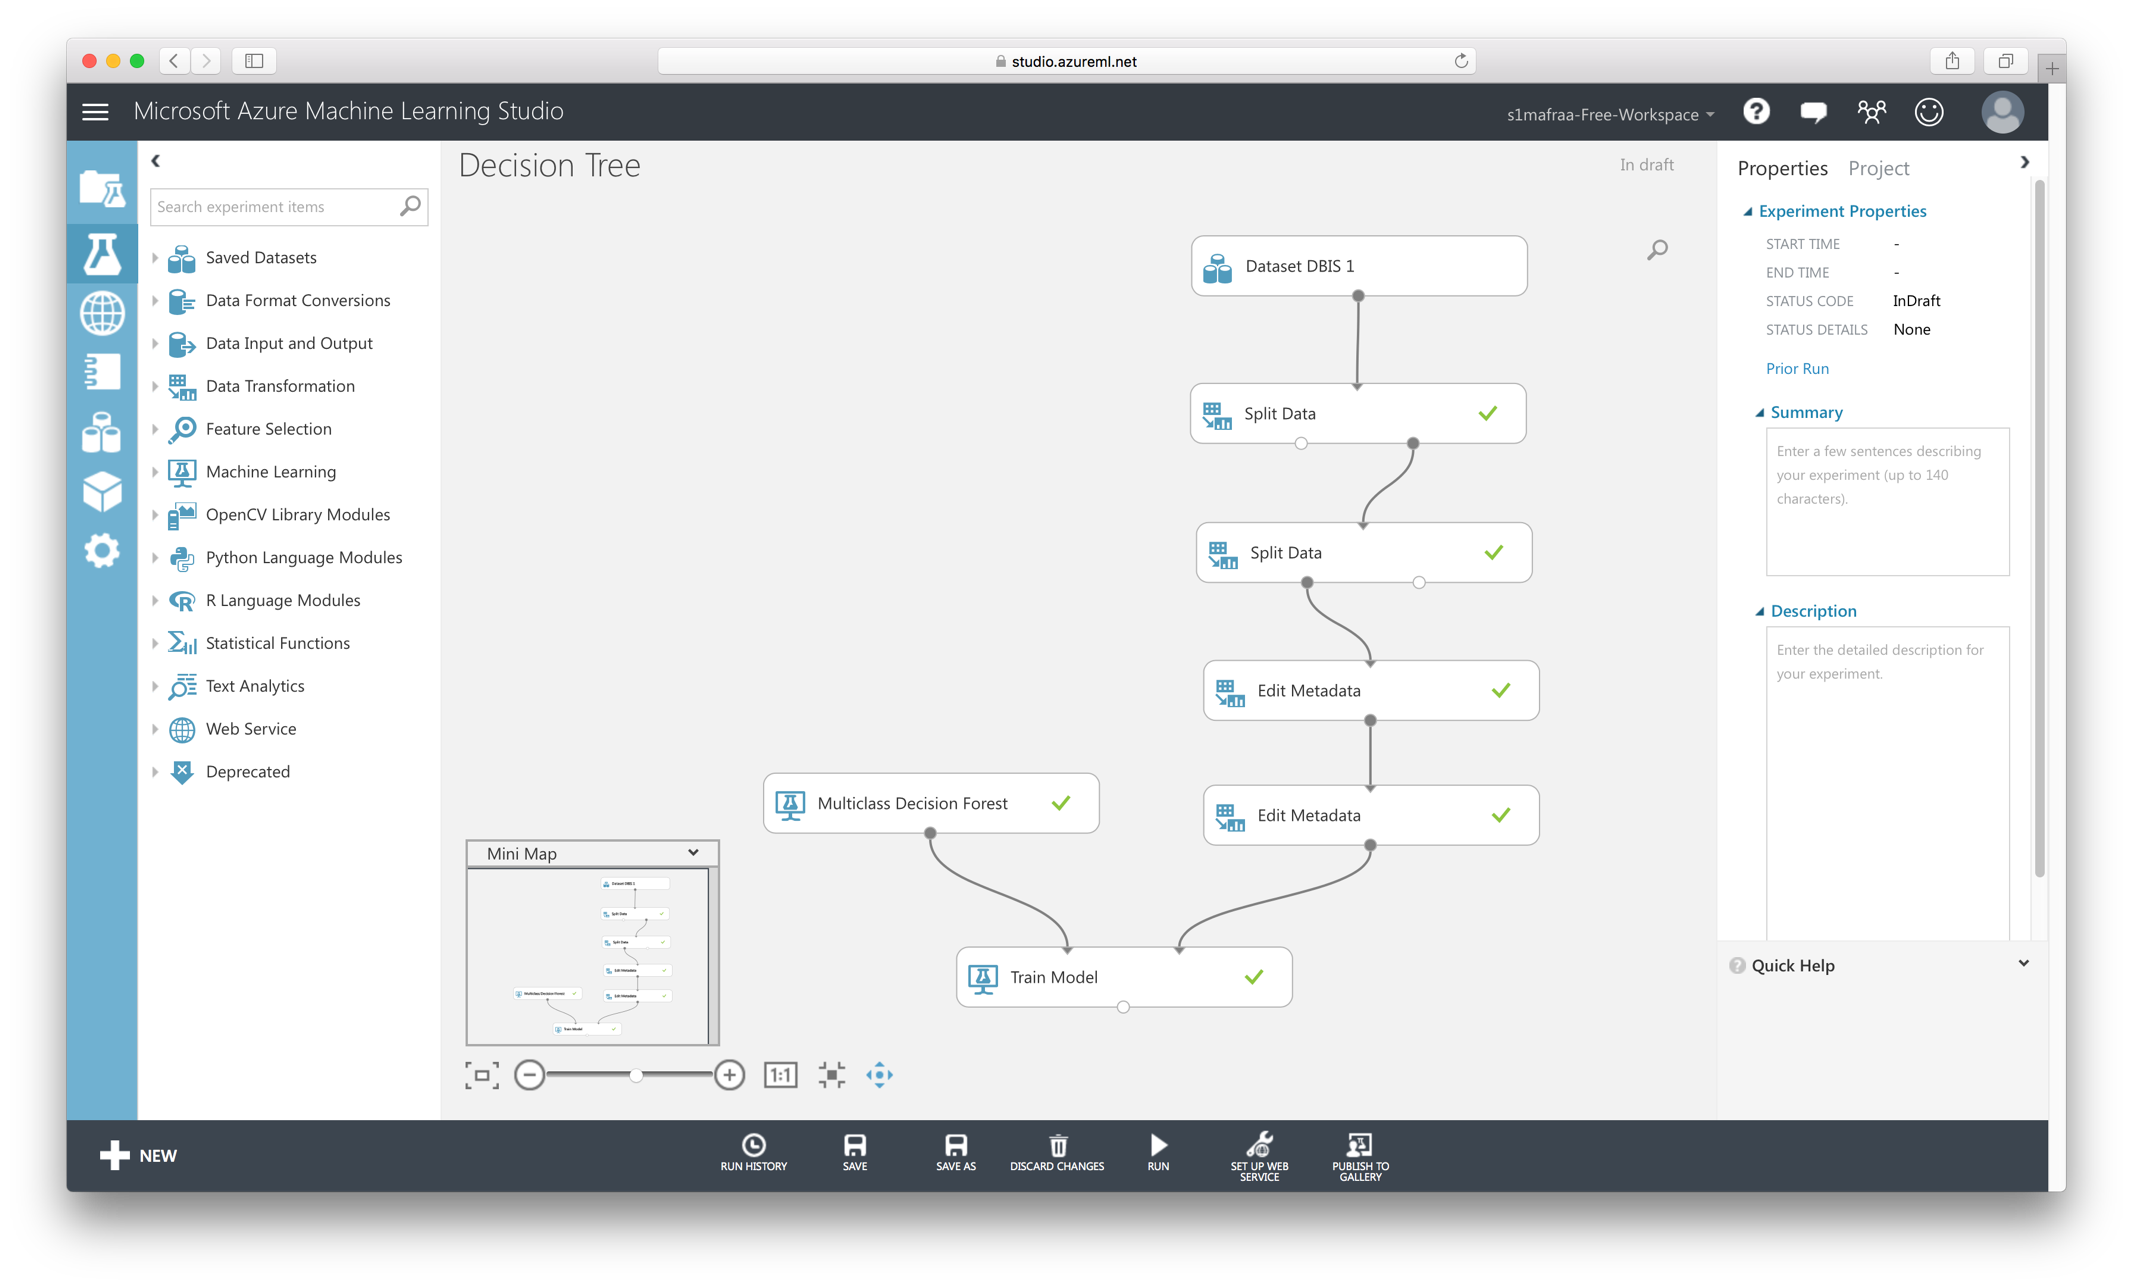
\includegraphics[width=0.85\textwidth]{gfx/msaproc.png}
	\caption{Das Beispiel-Experiment im Microsoft Azure Machine Learning Studio}
	\label{fig:example:impl:msa:proc}
\end{figure}

Hier fällt auf der rechten Seite auf, dass je 2 „Split Data“ und „Edit Metadata“
Operatoren gebraucht wurden. Um die selbe Filter-Funktionalität wie beim
RapidMiner Studio Prozess abzubilden, mussten zunächst alle NULL Einträge und
anschließend ebenfalls alle Datensätze, welche die Frage nach der Gesamtnote
beinhalten, herausgefiltert werden. Dafür waren hier 2 separate „Split“
Operationen notwendig. Des Weiteren wurde sowohl für die Definition des
Attributs „Answer“ als Label, als auch für die Definition der restlichen
Attribute als „klassifizierende Attribute“ je ein „Edit Metadata“ Operator
benötigt. Zuletzt fällt noch auf, dass anstatt eines Decision Tree Algorithmus
ein „Multiclass Decision Forest“, welcher als Konfiguration eine Decision-Tree
Anzahl von 1 bekommen hat, zur Berechnung verwendet wurde. Dies war notwendig,
um überhaupt ein auswertbares Ergebnis zu erhalten, welches zumindest
Ansatzweise mit dem Ergebnis des RapidMiner Studios vergleichbar ist.

\begin{figure}[htb]
  \center
	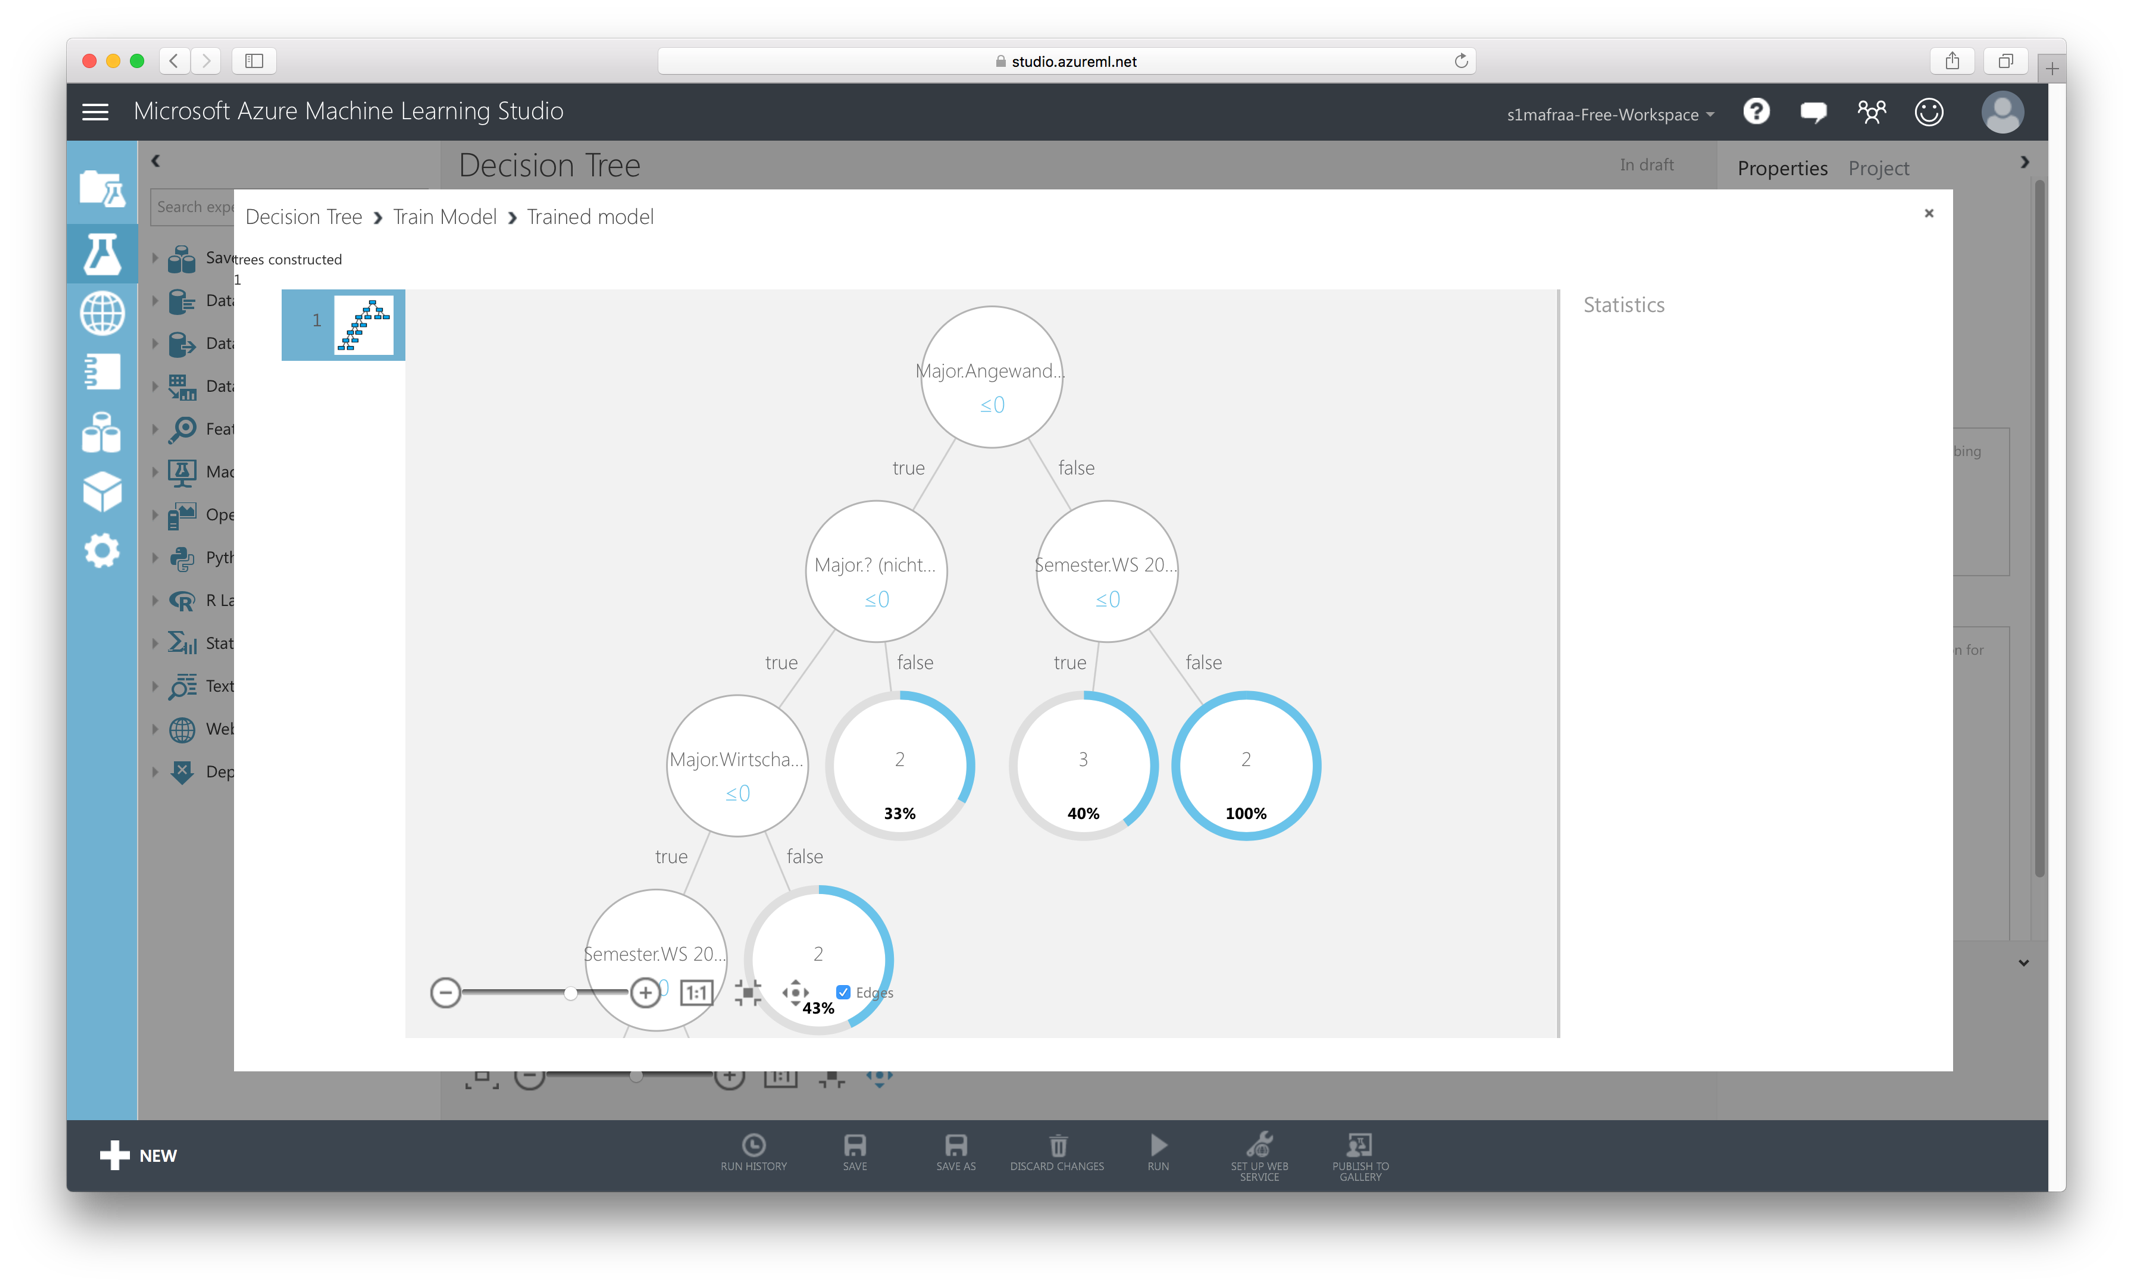
\includegraphics[width=0.85\textwidth]{gfx/msares.png}
	\caption{Das Ergebnis im Microsoft Azure Machine Learning Studio}
	\label{fig:example:impl:msa:res}
\end{figure}

Wie aufgrund der Tatsache, dass ein anderer Algorithmus verwendet wurde,
anzunehmen ist, weicht das Ergebnis vom vorherigen Ergebnis des RapidMiner
Studios in einigen Punkten ab. Der Baum zeigt, dass nicht zwangsläufig das
Studienfach ausschlaggebend für eine schlechtere Bewertung war, sondern das
Semester, in welchem die Umfrage durchgeführt wurde.
Auch hier lässt sich anhand der Blätter ablesen, wie groß die „Confidence“ der
jeweiligen Klasse ist. So lässt sich also interpretieren, dass Studierende, die
nicht dem „Major“ Angewandte Informatik angehören, dafür allerdings im
Wintersemester 2012/13 an der Umfrage teilgenommen haben überwiegend die Note
„3“ vergeben haben. Die Prozentzahl zeigt dabei an, dass 40\% der zugrunde
liegenden Datensätze in die Klasse „3“ fallen, wohingegen die anderen 60\%
sich auf die restlichen Werte 1, 2 bzw. 4, 5 und 6 verteilen.
